\documentclass{amsart}

\usepackage{tikz}
\usepackage{amsmath}
\usetikzlibrary{fit,arrows,calc,positioning,shapes}

\definecolor{heavyorange}{HTML}{FF7600}
\definecolor{almostblack}{HTML}{1a0f00}
\definecolor{lightorange}{HTML}{ffebcc}
\definecolor{lightgrey}{HTML}{f6f6f6}
\begin{document}
 
\begin{center}	
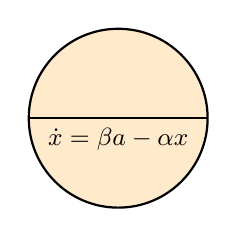
\begin{tikzpicture}
	 \begin{scope}[thick,font=\small]
	        
		\node[draw,circle split, thick, fill=lightorange](controller) 
					{\fontfamily{pcr}\selectfont \large  \nodepart{lower} $\dot{x}=\beta a - \alpha x$};
					
	 \end{scope}
\end{tikzpicture}
\end{center}

	
\end{document}